\section{Ewald summation}
\label{chap:ewald}

Within the Born-Oppenheimer approximation, the movement of the nuclei and the electrons is decoupled. This means that we can readily evaluate the electrostatic energy due to repelling nuclei via

\begin{equation}
    E_{\text{nuc-nuc}} = \frac{1}{2}\sum_{i}q_{i}\sum_{j \neq i,\vec{n}} \frac{q_{j}}{r_{ij} + \vec{n}},
    \label{eq:enucnuc}
\end{equation}

where $\vec{n}$ loops over all periodic images and the sum is evaluated for all particles except in the situation when $\vec{n} = \vec{0}$ and $i = j$. Due to the relatively slow decay of the $\frac{1}{r}$ term in \cref{eq:enucnuc}, this sum converges very slowly.\footnote{More technically, it is only conditionally convergent.}

As seen earlier in the derivation of $\nu_{\text{ext}}$, the charge density due to the nuclei can be represented by a sum of Dirac delta peaks and we can calculate the potential $\nu$ due to this set of point charges via the Poisson equation. This would yield the following equation for the total electrostatic repulsion between the nuclei.

\begin{equation}
    E_{\text{nuc-nuc}} = \frac{1}{2} \sum_{i} q_{i} \nu(\vec{R_{i}})
    \label{eq:enucnuc_realspace}
\end{equation}

Of course, this strategy does not circumvent the initial problem that the Coulombic potential is slowly decaying. To tackle this, we use a so-called Ewald summation wherein we introduce on top of the set of point charges a \textit{screening} diffuse charge cloud of opposite sign. For this \textit{screened} set of charges, its contribution to the potential $\nu$ is determined by the amount of charge that is unscreened, whose contribution will (very) rapidly decay with increasing distance. Of course, the introduction of the \textit{screening} charges adds a spurious contribution to the electrostatic potential, which must be compensated. This can be easily done by adding to the electrostatic potential a contribution of a compensating smoothly varying charge distribution, exactly opposite to the \textit{screening} charges. This is shown schematically in \cref{fig:ewald_schematic}.

\begin{Figure}
    \centering
    \resizebox{0.9 \textwidth}{!}{
        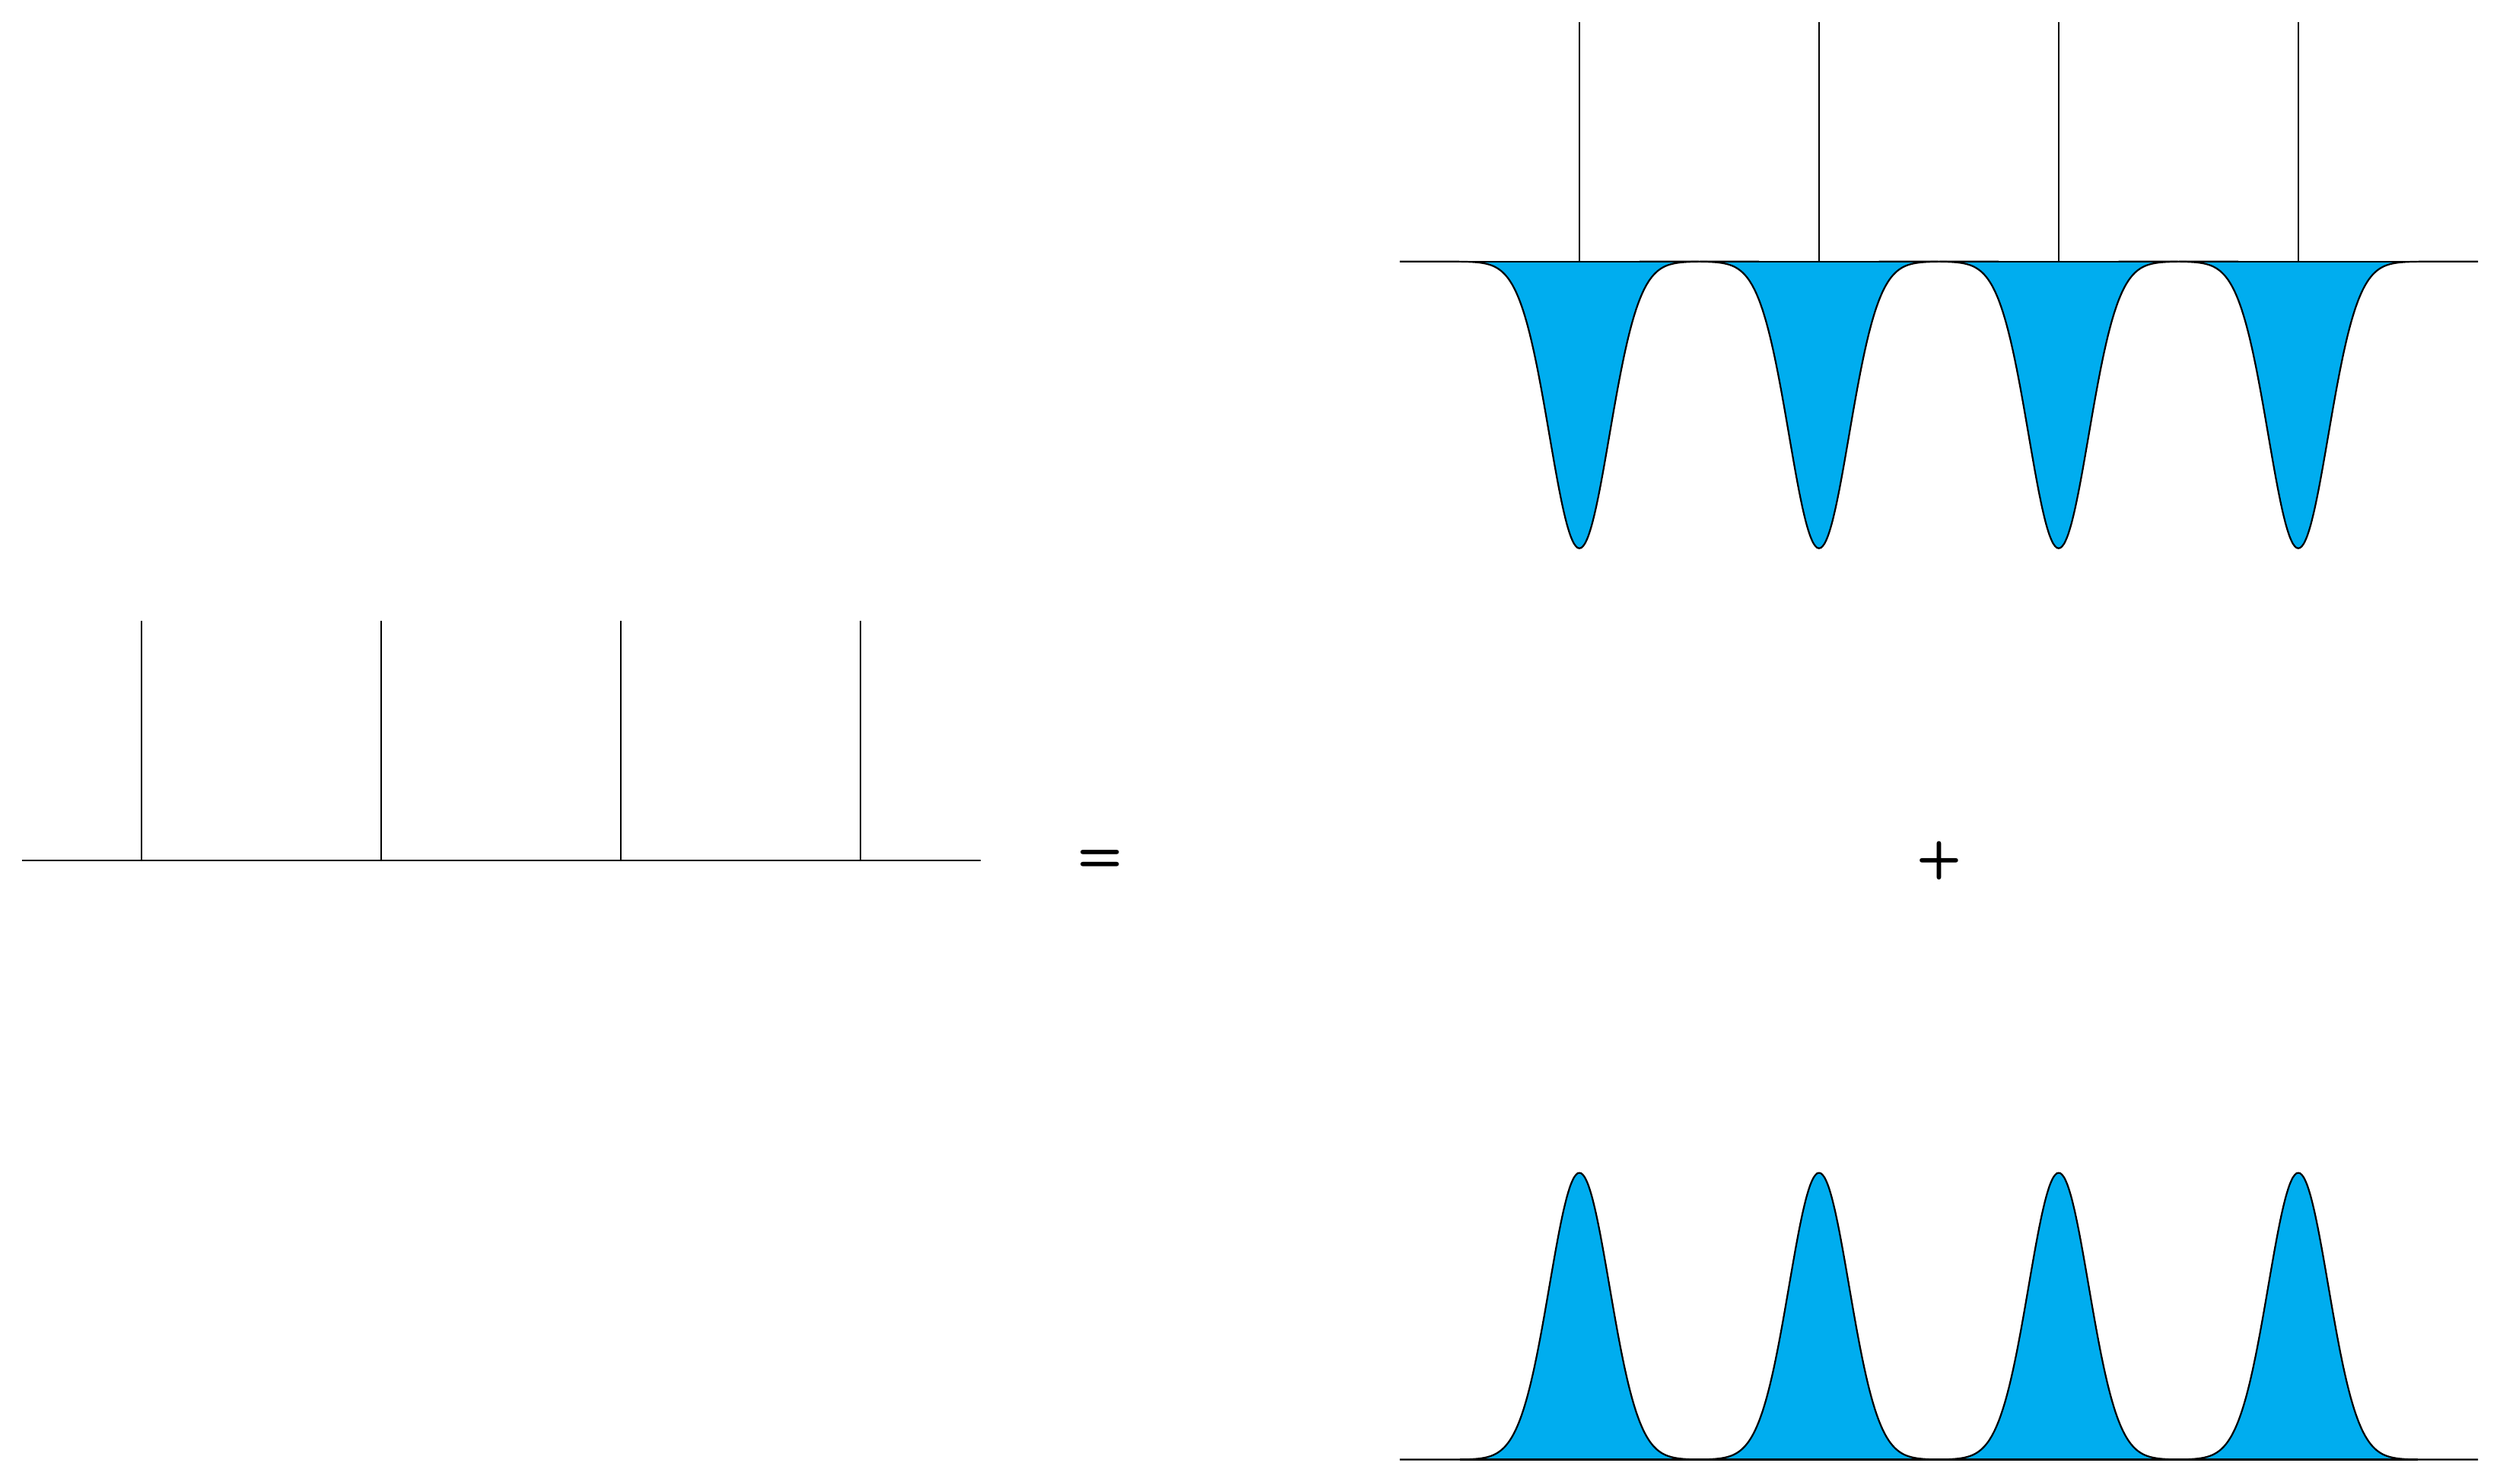
\begin{tikzpicture}
    % First filled Gaussian (centered at -6)
    \fill[cyan] plot[domain=-9:-3, samples=100] 
        ({\x}, {-12/(sqrt(2*pi))*exp(-2*(\x+6)^2)}) -- (-3,0) -- (-9,0) -- cycle;
    \draw[black, thick, smooth] plot[domain=-9:-3, samples=100] 
        ({\x}, {-12/(sqrt(2*pi))*exp(-2*(\x+6)^2)});\
    \draw[black, thick] (-6,0) -- (-6,4);
        
    % Second filled Gaussian (centered at -2)
    \fill[cyan] plot[domain=-5:1, samples=100] 
        ({\x}, {-12/(sqrt(2*pi))*exp(-2*(\x+2)^2)}) -- (1,0) -- (-5,0) -- cycle;
    \draw[black, thick, smooth] plot[domain=-5:1, samples=100] 
        ({\x}, {-12/(sqrt(2*pi))*exp(-2*(\x+2)^2)});
    \draw[black, thick] (-2,0) -- (-2,4);
    
    % Third filled Gaussian (centered at 2)
    \fill[cyan] plot[domain=-1:5, samples=100] 
        ({\x}, {-12/(sqrt(2*pi))*exp(-2*(\x-2)^2)}) -- (5,0) -- (-1,0) -- cycle;
    \draw[black, thick, smooth] plot[domain=-1:5, samples=100] 
        ({\x}, {-12/(sqrt(2*pi))*exp(-2*(\x-2)^2)});
    \draw[black, thick] (2,0) -- (2,4);
    
    % Fourth filled Gaussian (centered at 6)
    \fill[cyan] plot[domain=3:9, samples=100] 
        ({\x}, {-12/(sqrt(2*pi))*exp(-2*(\x-6)^2)}) -- (9,0) -- (3,0) -- cycle;
    \draw[black, thick, smooth] plot[domain=3:9, samples=100] 
        ({\x}, {-12/(sqrt(2*pi))*exp(-2*(\x-6)^2)});
    \draw[black, thick] (6,0) -- (6,4);

    \draw[black, thick] (-8,0) -- (8,0);

    % First filled Gaussian (centered at -6)
    \draw[black, thick] (-30,-10) -- (-30,-6);
        
    % Second filled Gaussian (centered at -2)
    \draw[black, thick] (-26,-10) -- (-26,-6);
    
    % Third filled Gaussian (centered at 2)
    \draw[black, thick] (-22,-10) -- (-22,-6);
    
    % Fourth filled Gaussian (centered at 6)
    \draw[black, thick] (-18,-10) -- (-18,-6);

    \draw[black, thick] (-32,-10) -- (-16,-10);

    \draw (-14,-10) node[font=\fontsize{80}{80}\sffamily\bfseries]{=};

    % First filled Gaussian (centered at -6, shifted downward by 20)
    \fill[cyan] plot[domain=-9:-3, samples=100] 
        ({\x}, {-20 + 12/(sqrt(2*pi))*exp(-2*(\x+6)^2)}) -- (-3,-20) -- (-9,-20) -- cycle;
    \draw[black, thick, smooth] plot[domain=-9:-3, samples=100] 
        ({\x}, {-20 + 12/(sqrt(2*pi))*exp(-2*(\x+6)^2)});
    
    % Second filled Gaussian (centered at -2, shifted downward by 20)
    \fill[cyan] plot[domain=-5:1, samples=100] 
        ({\x}, {-20 + 12/(sqrt(2*pi))*exp(-2*(\x+2)^2)}) -- (1,-20) -- (-5,-20) -- cycle;
    \draw[black, thick, smooth] plot[domain=-5:1, samples=100] 
        ({\x}, {-20 + 12/(sqrt(2*pi))*exp(-2*(\x+2)^2)});
    
    % Third filled Gaussian (centered at 2, shifted downward by 20)
    \fill[cyan] plot[domain=-1:5, samples=100] 
        ({\x}, {-20 + 12/(sqrt(2*pi))*exp(-2*(\x-2)^2)}) -- (5,-20) -- (-1,-20) -- cycle;
    \draw[black, thick, smooth] plot[domain=-1:5, samples=100] 
        ({\x}, {-20 + 12/(sqrt(2*pi))*exp(-2*(\x-2)^2)});
    
    % Fourth filled Gaussian (centered at 6, shifted downward by 20)
    \fill[cyan] plot[domain=3:9, samples=100] 
        ({\x}, {-20 + 12/(sqrt(2*pi))*exp(-2*(\x-6)^2)}) -- (9,-20) -- (3,-20) -- cycle;
    \draw[black, thick, smooth] plot[domain=3:9, samples=100] 
        ({\x}, {-20 + 12/(sqrt(2*pi))*exp(-2*(\x-6)^2)});

    \draw[black, thick] (-8,-20) -- (8,-20);

    \draw (0,-10) node[font=\fontsize{80}{80}\sffamily\bfseries]{+};

\end{tikzpicture}
    }
    \captionof{figure}{A set of points charges (left) can be described as a set of screened charges (right top) minus a smoothly varying compensating charge distribution of opposite sign (right bottom).}
    \label{fig:ewald_schematic}
\end{Figure}

The interaction of the electrostatic potential due to the combination of the \textit{screened} and \textit{compensating} charge distributions should only be evaluated for those \textit{screening} and \textit{compensating} charges that are spawned by the nuclei $j \neq i$. It turns out however that it is convenient to include the spurious self-interactions between the \textit{compensating} charge cloud and the nuclei. By doing so, the compensating charge cloud is a periodic function, allowing us to represent it by a series of plane waves and utilizing the Poisson equation to calculate the potential. It does imply that we need to correct for the spurious self-interaction.

Summarizing, $\nu$ can be decomposed into three terms,

\begin{enumerate}
    \item A long-range contribution due to the \textit{compensating} charge cloud: $\nu_{\text{lr}}$
    \item A short-range contribution due to the \textit{screened} charges: $\nu_{\text{sr}}$
    \item A correction term for the on-site spurious self-interaction: $\nu_{\text{s}}$.
\end{enumerate}

It should be mentioned that the Ewald procedure as shown above can formally only be applied to neutral systems, which our system is not. As such, we have to apply one more correction, a so-called electroneutrality term, which is explained in \cref{sec:electroneutrality}.

%
%
%
\subsection{Long-range contribution}

We start by deriving an expression for $\nu_{\text{lr}}$. For the smoothly varying \textit{compensating} charge density, a Gaussian is used

\begin{equation}
    \rho_{j}(\vec{r}) = q_{j} \left( \frac{\alpha}{\pi} \right)^{3/2} \exp \left(- \alpha \left|\vec{r} - \vec{R}_{j} \right|^{2} \right)
    \label{eq:gaussian}
\end{equation}

such that the \textit{compensating} charge density $\rho_{c}(\vec{r})$ is given by

\begin{equation}
    \rho_{c}(\vec{r}) = \sum_{j} q_{j} \left( \frac{\alpha}{\pi} \right)^{3/2} \exp \left(- \alpha \left|\vec{r} - \vec{R}_{j} \right|^{2} \right).
    \label{eq:ewald_charge_dens}
\end{equation}

and wherein the value of $\alpha$ is chosen such that the Gaussian effectively screens the charge. More details on how to determine the appropriate value of $\alpha$ is provided in \cref{sec:est_ewald}.

The Fourier transform of the charge density shown in \cref{eq:ewald_charge_dens} can be found by solving

\begin{align}
    \rho_{c}(\vec{G}) &= \frac{1}{\sqrt{\Omega}}\int_{\Omega} d\vec{r} \; \exp\left(-i\vec{G} \cdot \vec{r} \right) \sum_{j} q_{j} \left( \frac{\alpha}{\pi} \right)^{3/2} \exp \left(- \alpha \left|\vec{r} - \vec{R}_{j} \right|^{2} \right) \\
    &= \frac{1}{\sqrt{\Omega}} \sum_{j} q_{j} \exp \left(-i \vec{G} \cdot \vec{R}_{j} \right) \exp \left(- \frac{|\vec{G}|^{2}}{4 \alpha} \right)
\end{align}

By application of \cref{eq:poisson}, the reciprocal-space representation of the electrostatic potential due to the \textit{compensating} charges corresponds to

\begin{equation}
    \nu_{\text{lr}}(\vec{G}) = \frac{4\pi}{|\vec{G}|^{2}\sqrt{\Omega}} \sum_{j} q_{j} \exp \left(-i \vec{G} \cdot \vec{R}_{j} \right) \exp \left(- \frac{|\vec{G}|^{2}}{4 \alpha} \right).
    \label{eq:nulr-g}
\end{equation}

Finally, from \cref{eq:enucnuc_realspace} we can calculate the electrostatic \textbf{energy} by application of \cref{eq:plane-wave-exp} to \cref{eq:nulr-g}, yielding

\begin{equation}
    E_{\text{lr}} = \frac{2 \pi}{\Omega} \sum_{\vec{G} \neq 0} \sum_{i,j} \frac{q_{i}q_{j}}{|\vec{G}|^{2}} \exp \left(i \vec{G} \cdot \left(\vec{R}_{i} - \vec{R}_{j} \right) \right) \exp \left(- \frac{|\vec{G}|^{2}}{4 \alpha} \right). \label{eq:long-range}
\end{equation}

Observe that in \cref{eq:long-range}, the divergent term corresponding to $\vec{G} = \vec{0}$ has been omitted. Furthermore, if we assume that any imaginary terms can be ignored, \cref{eq:long-range} can be further simplified to

\begin{equation}
    E_{\text{lr}} = \frac{2 \pi}{\Omega} \sum_{\vec{G} \neq 0} \sum_{i,j} \frac{q_{i}q_{j}}{|\vec{G}|^{2}} \cos \left(\vec{G} \cdot \vec{R}_{ij} \right) \exp \left(- \frac{|\vec{G}|^{2}}{4 \alpha} \right),
    \label{eq:long-range-cos}
\end{equation}

where $\vec{R}_{ij}$ is shorthand for $\vec{R}_{i} - \vec{R_{j}}$.

%
%
%
\subsection{Self-interaction term}

We continue by calculating the self-interaction term as part of the derivation shown here can be reused in the derivation of the short-range interaction. The self-interaction term is due to the \textit{screening} charge of opposite sign with a point charge. We first calculate the potential due to the screening charge. Application of \cref{eq:poisson} to \cref{eq:gaussian}, noting the spherical symmetry and taking $\vec{R} = \vec{0}$ yields the following second order differential equation

\begin{equation}
    \nabla^{2} \nu_{\text{s}} (r) = -4 \pi q_{j} \left( \frac{\alpha}{\pi} \right)^{3/2} \exp \left(- \alpha r^{2} \right)
\end{equation}

Two-fold partial integration of the above equation yields

\begin{equation}
    \nu_{\text{s}} (r) = \frac{q_{i}}{r} \erf \left( \sqrt{\alpha} r \right),
    \label{eq:gaussian_erf}
\end{equation}

where $\erf()$ represents the error function. At $r = 0$, the above function evaluates to

\begin{equation}
    \nu_{\text{s}} (0) = 2 q_{i} \sqrt{\frac{\alpha}{\pi}},
\end{equation}

such that

\begin{align}
    E_{\text{s}} &= \frac{1}{2} \sum_{i} q_{i} \cdot \nu_{\text{s}} (0) \\
    &= \sqrt{\frac{\alpha}{\pi}} \sum_{i} q_{i}^{2}.
    \label{eq:ewald_self}
\end{align}

%
%
%
\subsection{Short-range contribution}

The last term corresponds to the short-range contribution of the \textit{screened} charges. The electrostatic potential due to the \textit{screened} charges is the combination of the contributions due to the \textit{screening} Gaussian charge and the point charge, the former corresponding to the result as found in \cref{eq:gaussian_erf}. For the combination, we find

\begin{align}
    \nu_{\text{sr}} &= \sum_{j} \frac{q_{j}}{r} - \frac{q_{j}}{r} \erf \left( \sqrt{\alpha} r \right) \\
    &= \sum_{j} \frac{q_{j}}{r} \erfc \left( \sqrt{\alpha} r \right),
    \label{eq:nu_shortrange}
\end{align}

where $\erfc()$ corresponds to the complementary error function. The total electrostatic energy due to the \textit{screened} charges is thus

\begin{equation}
    E_{\text{sr}} = \frac{1}{2} \sum_{\vec{n} \neq \vec{0}} \sum_{i \neq j} \frac{q_{i}q_{j}}{|\vec{r}_{ij} + \vec{n}|} \erfc \left( 
\sqrt{\alpha} |\vec{r}_{ij} + \vec{n}| \right)
\label{eq:ewald_sr}
\end{equation}

In \cref{sec:est_ewald}, it will be explained how to determine which values of $\vec{n}$ to use in the expansion as shown in \cref{eq:ewald_sr}.

%
%
%
\subsection{Electroneutrality term}
\label{sec:electroneutrality}

In the above derivation, we removed the divergent $\vec{G}=\vec{0}$ term in the calculation of the long-range interaction. We are allowed to do so for neutral systems as in that circumstance the term would cancel out, yet the set of nuclei is \textbf{not} a neutral system. We thus have to apply another correction, corresponding to the spurious removal of charge density corresponding to the $\vec{G}=\vec{0}$ term, i.e. $\tilde{\rho}(\vec{G}=\vec{0})$, which corresponds to

\begin{equation}
    \tilde{\rho}(\vec{G}=\vec{0}) = \sum_{j}q_{j}.
\end{equation}

The electroneutrality term ($E_{\text{en}}$) can be readily evaluated in real-space by calculating the interaction of the \textit{screened} charges with a uniform background charge as given by

\begin{equation}
    \rho_{\text{bg}} = \frac{\sum_{i}q_{i}}{\Omega}.
\end{equation}

giving the following result

\begin{align}
    E_{\text{en}} &= \frac{1}{2} \int_{\Omega} d\vec{r} \; \rho_{\text{bg}} \nu_{\text{sr}} \\
    &= \frac{\sum_{i,j}q_{i}q_{j}}{\Omega} \int_{\Omega} d\vec{r} \; \frac{1}{r} \erfc \left( \sqrt{\alpha} r \right) \\
    &= \frac{\pi}{2 \alpha \Omega} \left(\sum_{i} q_{i} \right)^{2}
    \label{eq:ewald_en}
\end{align}

Having all terms established, the Ewald energy is essentially the sum of the short- and long-range interactions (\cref{eq:long-range-cos,eq:ewald_sr}) with an additional self-interaction and electroneutrality correction (\cref{eq:ewald_self,eq:ewald_en}) yielding

\begin{equation}
    E_{\text{Ewald}} = E_{\text{sr}} + E_{\text{lr}} - E_{\text{s}} - E_{\text{en}}.
\end{equation}

%
%
%
\subsection{Establishing Ewald sum parameters}
\label{sec:est_ewald}

The above procedure utilizes the term $\alpha$ to specify the width of the Gaussian and $\vec{n}$ to indicate the number neighboring unit cells considered in the short-range expansion. Furthermore, no cut-off energy is provided for plane waves used in the long-range expansion. Below, a brief recipe is provided to estimate their values.

First, we introduce the parameter $\gamma$ from which, together with the cut-off energy $E_{\text{cut}}$, the value for $\alpha$ can be derived via

\begin{equation}
    \alpha = -\frac{1}{4} \frac{E_{\text{cut}}^{2}}{\ln \gamma}.
    \label{eq:alpha_ewald}
\end{equation}

Next, to construct the set $\{\vec{n}\}$, the maximum value for $N_{i} = \max\left(|n_{i}|\right)$ for each lattice vector $\vec{a}_{i}$ is established by means of

\begin{equation}
    N_{i} = \nint*{-\frac{1}{2 |a_{i}|} \frac{\ln \gamma}{\sqrt{\alpha}} + \frac{3}{2}}
\end{equation}

where $\nint{x}$ represents the rounding of $x$ to its nearest integer. Using $N_{i}$, the set $\{n_{i} / |\vec{a}_{i}|\}$ runs according to

\begin{equation}
    -N_{i}, -N_{i} + 1, \cdots, N_{i}-1, N_{i}.
    \label{eq:iteration_ewald}
\end{equation}

Finally, a similar procedure is applied to determine the set of plane waves used to calculate the long-range interaction. The maximum value for $M_{i} = \max\left(|G_{i}|\right)$ is given by

\begin{equation}
    M_{i} = \nint*{\frac{E_{\text{cut}}}{|\vec{b}_{i}|} + \frac{3}{2}}
\end{equation}

such that $G_{i} / |\vec{b}_{i}|$ runs according to \cref{eq:iteration_ewald}.

Finally, recommended values for $\gamma$ and $E_{\text{cut}}$ correspond to

\begin{align}
    \gamma &= 10^{-8}\\
    E_{\text{cut}} &= 2 \; \text{Ht}.
\end{align}

Note that $E_{\text{cut}}$ effectively acts as a splitting parameter between the short-range and long-rage parts of the Ewald summation. The value of $E_{\text{cut}} = 2$ Ht is chosen such that this division ensures an efficient computation. To illustrate this, for a cubic unit cell with dimensions $10 \times 10 \times 10$ a.u., with a value of $E_{\text{cut}} = 2$ Ht yields $N_{i} = 3$ and $M_{i} = 5$. A much smaller value of $E_{\text{cut}} = 0.1$ Ht yields $N_{i} = 28$ and $M_{i} = 2$ and a much larger value of $E_{\text{cut}} = 10.0$ Ht gives yields $N_{i} = 2$ and $M_{i} = 17$. From this example, we can see that lowering $E_{\text{cut}} = 2$ Ht increases the number of neighboring unit cells taken into account in the short-range sampling while reducing the number of plane waves in the long-range sampling. Contrariwise, increasing the value reduces the computation time for the short-range sampling, but leads to increased computation times for the long-range interaction. The value $E_{\text{cut}} = 2$ Ht is a compromise such that relatively optimal computation times are achieved.